\documentclass[xcolor=dvipsnames, aspectratio = 169]{beamer}
\usepackage[english]{babel} %% english
\usepackage[utf8]{inputenc}
\usepackage[T1]{fontenc}
\usepackage{include/chariteBeamer}
\usepackage{hyperref}
\input{include/header2}
\tikzset{>=latex}
%\usepackage{amsmath}
%\usetikzlibrary{shadows}
\usepackage[edges]{forest}
\usetikzlibrary{positioning}
\usepackage{biostat}
\setbeamertemplate{caption}[numbered]
\let\qed\relax
\forestset{declare toks={elo}{}}
%% ================================================================== %% 

\author[E. Sprünken]{Erin Sprünken} 
\title{Non-parametric procedures for clustered data in the several sample case} 
\date[]{\today}

%% ================================================================== %% 
\setbeamercolor*{mycol}{bg=chariteGray, fg=chariteBlue}

\hyphenation{Sam-ples}
\begin{document}

%% ================================================================== %%
%% ================================================================== %%
\setbeamertemplate{footline}{\begin{tikzpicture}
    \node [inner sep=0pt, anchor=east] (0,0) {
      \includegraphics[width=\paperwidth,height=0.7cm]{include/charite_footer}};
    \node [inner sep=0pt, anchor=east] at (-0.5ex,-0ex){};
\end{tikzpicture}}

\setbeamertemplate{headline}{
%\leavevmode
\hspace{-0.49em}\hbox{
	\begin{beamercolorbox}[wd=1.02\paperwidth,ht=2.25ex,dp=1ex,left]{mycol}%
    \usebeamerfont{section in head/foot}
  \end{beamercolorbox}%
}}
{
  \usebackgroundtemplate{ \hspace{-0.5em}\begin{tikzpicture}
  \node[opacity=0.7, anchor=south] (0,0) {\includegraphics[height=\paperheight, width=1.04\paperwidth]{include/frontmatter.pdf}};
  \end{tikzpicture}
} 
%\frame{\titlepage}
\begin{frame}
\centering
	\vspace{4em}
	{\Large \textcolor{chariteBlue}{\inserttitle}}\\
	 \vspace{1em}
	{\Large \textcolor{black}{\insertauthor \\}} 
	\vspace{2em}
	{\footnotesize \textcolor{black}{\insertinstitute \\\vspace{1em} \insertdate}} 
	\vspace{0em}
	\begin{figure}[h!]
		\includegraphics[width=5cm]{include/Charite_Logo.png}
	\end{figure}
%	\pgfuseimage{frontUnilogo}
\end{frame}
}
%% ================================================================== %%

\setbeamertemplate{footline}{\begin{tikzpicture}
    \node [inner sep=0pt, anchor=east] (0,0) {
      \includegraphics[width=\paperwidth,height=0.7cm]{include/charite_footer}};
    \node [inner sep=0pt, anchor=east] at (-0.5ex,-0ex) {\tiny \insertframenumber{}$\,$|$\,$\inserttotalframenumber};
\end{tikzpicture}}

\setbeamertemplate{headline}{%
%\leavevmode%
\hspace{-0.49em}\hbox{
	\begin{beamercolorbox}[wd=.78\paperwidth,ht=2.25ex,dp=1ex,left]{mycol}%
    \usebeamerfont{section in head/foot}\hspace*{1em}
  \end{beamercolorbox}%
  \begin{beamercolorbox}[wd=.10\paperwidth,ht=2.25ex,dp=1ex,right]{mycol}%
    \usebeamerfont{author in head/foot}\insertshortauthor
  \end{beamercolorbox}%
  \begin{beamercolorbox}[wd=.14\paperwidth,ht=2.25ex,dp=1ex,center]{mycol}%
    \usebeamerfont{date in head/foot}\insertdate
  \end{beamercolorbox}%
  }
}


\frame{\tableofcontents}

\setbeamertemplate{headline}{%
%\leavevmode%
\hspace{-0.49em}\hbox{
	\begin{beamercolorbox}[wd=.78\paperwidth,ht=2.25ex,dp=1ex,left]{mycol}%
    \usebeamerfont{section in head/foot}\hspace*{1em}\thesection. \  \insertsectionhead
  \end{beamercolorbox}%
  \begin{beamercolorbox}[wd=.10\paperwidth,ht=2.25ex,dp=1ex,right]{mycol}%
    \usebeamerfont{author in head/foot}\insertshortauthor
  \end{beamercolorbox}%
  \begin{beamercolorbox}[wd=.14\paperwidth,ht=2.25ex,dp=1ex,center]{mycol}%
    \usebeamerfont{date in head/foot}\insertdate
  \end{beamercolorbox}%
  }
}

\section{Introduction}
\begin{frame}[fragile]{Motivation}
  \begin{itemize}
  \item Clustered data describes data, where observations consist of potentially correlated subobservations.
  \item In many experiments and trials, such data can occur, for example pupils of the same class or mice sharing the same cage. 
  \item Typically, assumptions about scale, distributions and correlation structure are hard to justify in practice.
  \end{itemize}
%  \begin{tikzpicture}
%  [[level distance=11mm,
%  every node/.style = {shape=rectangle, rounded corners,
%    draw, align=center,
%    top color=white, bottom color=blue!20}]]
%  \node {Sample}
%		child { node {Group 1} }
%		child { node {Group i}
%			child { node {Observation 1 (Cluster 1)} }
%			child { node {Observation j (Cluster j)} }
%			child { node {Observation $n_i$ (Cluster $n_i$)} }
%		 }
%		child { node {Group n} };
%\end{tikzpicture}
\end{frame}
\begin{frame}[fragile]{Data Structure}
%\begin{forest}
%for tree={s sep+=3.9em,circle,draw,inner sep=1pt,
%    where n children=0{fill=white}{fill=black},
%    decision edge label/.style n args=3{
%    edge label/.expanded={node[midway,auto=#1,anchor=#2,\forestoption{elo}]{\strut$#3$}}
%  },
%  decision/.style={if n=1
%    {decision edge label={left}{east}{#1}}
%    {decision edge label={right}{west}{#1}}
%  },
%    }
% [,label=above:{Samples}
%  [,label=above:{Group $1$}
%   %[,label=above:{Cluster $[1,n_1]$}
%    %[,label=below:{Obs $1$}]
%    %[,label=below:{Obs $k$}]
%    %[,label=below:{Obs $n_{11m}$}]
%   %]
%  ]
%  [,label=above:{Group $i$}
%	[,label=above:{Cluster $1$}
%    	[,label=below:{Obs $1$}]
%    	[,label=below:{Obs $k$}]
%    	[,label=below:{ Obs $m_{i1}$ }]
%    ]
%   	[,label=above:{Cluster $j$}
%    	[name=X,label=below:{Obs $1$}] % \tikz{\node[] (unsichtbarenode1) {};}
%    	[name=Y,label=below:{Obs $k$}] % \tikz{\node[] (unsichtbarenode2) {};}
%    	[,label=below:{Obs $m_{ij}$}]
%    	
%    ]
%   	[,label=above:{Cluster $n_i$}
%    	[,label=below:{Obs $1$}]
%    	[,label=below:{Obs $k$}]
%   		[,label=below:{Obs $m_{in_i}$}]
%    ]
%  ]
%  [,label=above:{Group $d$}
%   %[,label=above:{Cluster $[1,n_n]$}
%    %[,label=below:{Obs $1$}]
%    %[,label=below:{Obs $k$}]
%    %[,label=below:{Obs $n_{11m}$}]
%   %]
%  ]
% ]
% %\draw (Y.south) -- (X.south);
%\end{forest}
\begin{center}
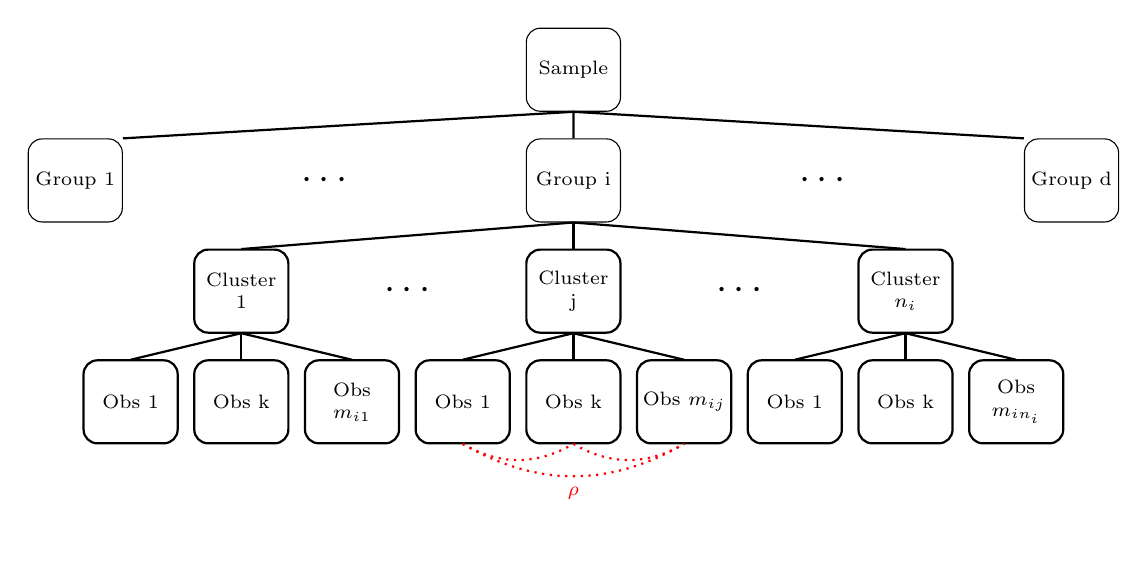
\begin{tikzpicture}[align=center, parent anchor=south,child anchor=north,grow=south, level 1/.style={sibling distance=9em, level distance = 4em},
level 2/.style={sibling distance=6em}, 
level 3/.style={sibling distance=4em}, level distance = 5em]
%\tikzset{every node/.style={ball color=orange,circle,text=white}}
\tikzset{every node/.style={rectangle, draw=black, rounded corners=0.5em, inner sep=2pt, minimum size = 3em, text width=3em, font=\scriptsize},
level 4/.style={rectangle, draw=none, level distance=3.3em, text=red}}
\tikzset{edge from parent/.style={draw,solid,thick,black}}
\node {Sample}
	child {node (v1){Group 1} edge from parent[child anchor=north east]}
	child {node[draw=none] (v1left){\Large $\cdots$} edge from parent[draw=none]}
	child {node (v2){Group i}
		child {node (v11){Cluster 1}
			child {node (v111){Obs 1}}
			child {node (v112){Obs k}}
			child {node (v113){Obs $m_{i1}$}}
		}
		child {node[draw=none] (v11left){\Large $\cdots$} edge from parent[draw=none]}
		child {node (v12){Cluster j}
			child {node (v121){Obs 1}}
			child {node (v122){Obs k}
				child {node[draw=none] (v1221){$\rho$} edge from parent[draw=none]}			
			}
			child {node (v123){Obs $m_{ij}$}}
		}
		child {node[draw=none] (v11right){\Large $\cdots$} edge from parent[draw=none]}
		child {node (v13){Cluster $n_i$}
			child {node (v131){Obs 1}}
			child {node (v132){Obs k}}
			child {node (v133){Obs $m_{in_i}$}}
		}
	}
	child {node[draw=none] (v1rightt){\Large $\cdots$} edge from parent[draw=none]}
	child {node (v3){Group d} edge from parent[child anchor=north west]}
;
\path[draw=red,dotted, thick] (v121.south)  edge[bend right](v122.south);
\path[draw=red,dotted, thick] (v122.south) edge[bend right](v123.south);
\path[draw=red,dotted, thick] (v121.south) edge[bend right](v123.south);
%\path[draw=black, dotted,very thick] (v1.east) edge (v2.west);
%\path[draw=black, dotted,very thick] (v2.east) edge (v3.west);
%\draw

\end{tikzpicture}
\end{center}
\end{frame}
\begin{frame}{Previous Works}
	\begin{itemize}
		\item Under assumption of Normality, Mixed Models are used, see Laird and Ware (1982) and Molenberghs and Verbeke (1997)
		\item For two samples and binary clustered data a $\chi^2$-test for contingency tables is used, see Jung et al. (2003)
		\item For two samples and assumption of equal distribution,  a generalization of the Wilcoxon-Mann-Whitney-test is used, see Datta and Satten (2005), Rosner et al. (2006) and Dutta and Datta (2016)
		\item For two samples and assumption of equal Wilcoxon-Mann-Whitney effects, see Roy et al. (2019)
	\end{itemize}
	We pick up the last point and generalize their procedure to a general framework for the several sample case under mild assumptions.
\end{frame}

%% ================================================================== %%
\section{Methodology}
\subsection*{Asymptotic Results}
\begin{frame}{Notation and Definition}
	\begin{itemize}
		\item The observation $k$ of group $i$ within a cluster $j$ follows a marginal distribution $F_i$: $X_{ijk} \thicksim F_i$ 
		\item The distribution function $F_i(x)$ is normalized, i.e. $F_i(x) = 0.5 \cdot [F_i^{-}(x) + F_i^{+}(x)]$ 
		\item $F_i^{-}(x) = \Pm{X_{ijk} < x}$ and $F_i^{+}(x) = \Pm{X_{ijk} \leq x}$
		\item We define a distribution function for group $i$ as $F_i^{\bm{\psi}} = \sum_{j=1}^{n_i}\sum_{k=1}^{m_{ij}}\psi_{ij}m_{ij}^{-1} F_i(x)$
		\item We define a reference distribution function as $F_{\bm{\theta}}(x) = \sum_{i=1}^d \theta_i F_i^{\bm{\psi}}(x)$
		\item The nonparametric relative effect for group $i$ is defined as $p_i = \int F_{\bm{\theta}}\dif F_i^{\bm{\psi}}$
		\item The weights $\bm{\theta}$ and $\bm{\psi}$ are normalized, such that $\sum_{i=1}^d \theta_i = 1$ and $\sum_{j=1}^{n_i}\sum_{k=1}^{m_{ij}} \psi_{ij} = 1$.
	\end{itemize}
\end{frame}

\begin{frame}{Asymptotic Equivalence}
	We showed that $\sqrt{g(n)}(\widehat{\bm{p}} - \bm{p}) \cdis N(\bm{0}, \bm{\Sigma})$ by using asymptotic equivalence:\\
	$$\forall i: \qquad \widehat{p}_i - p_i \quad \aseq \quad \int F_{\bm{\theta}} \dif \widehat{F}_i^{\bm{\psi}} - \int F_i \dif \widehat{F}_{\bm{\theta}} + 1 - 2p_i + A_i,$$ where
	$$\sqrt{g(n)}A_i \quad \clp \quad 0.$$
\end{frame}
\begin{frame}{Asymptotic Equivalence}
	For technical reasons, we use a different formulation of the former:
	\begin{equation*}
	\sqrt{g(n)}\left(\widehat{\vc{p}} - \vc{p}\right) \quad \aseq \quad \sqrt{g(n)} \sum_{i=1}^d\sum_{j=1}^{n_i} \psi_{ij} \vc{A}_{ij},
\end{equation*}
where \begin{align*}
	\vc{A}_{ij} \quad &= \quad \left(A_{hij}\right)_{h \in (1,...,d)} \\
	A_{hij} \quad &= \quad \begin{cases}
		\sum_{\substack{s=1 \\ s \neq i}}^d \theta_s Y_{ij}^{(s)} &\quad h = i \\
	- \theta_i Y_{ij}^{(h)} &\quad h \neq i.
	\end{cases} \\
	Y_{ab}^{(c)} \quad &= \quad \sum_{k=1}^{m_{ab}} \frac{1}{m_{ab}}F_{c}(X_{abk})
\end{align*}
\end{frame}

\subsection*{Variance-Covariance}
\begin{frame}{(Unobservable) Variance Estimator}
We propose the following:
\begin{align*}
	\overline{\vc{A}}_{i\cdot}^{*} \quad &= \quad \sum_{j=1}^{n_i} \psi_{ij}\vc{A}_{ij} \\
	\widehat{\bm{\Sigma}}_{ij}^{*} \quad &= \quad \left(\vc{A}_{ij} - \overline{\vc{A}}_{i\cdot}^{*}\right)\left(\vc{A}_{ij} - \overline{\vc{A}}_{i\cdot}^{*}\right)^{\intercal} \\
	\widehat{\bm{\Sigma}}^{u*} \quad &= \quad g(n)\sum_{i=1}^d\sum_{j=1}^{n_i}\psi_{ij}^2 \widehat{\bm{\Sigma}}_{ij}^{*}.
\end{align*}
However, this estimator is biased. Solution?
\end{frame}
\begin{frame}{Bias Correction}
An unbiased estimator is given by
\begin{equation*}
	\widehat{\bm{\Sigma}}^{*} \quad = \quad g(n)\sum_{i=1}^d\sum_{j=1}^{n_i} \psi_{ij}^2 \kappa_{ij}^{-1} \widehat{\bm{\Sigma}}_{ij}^{*},
\end{equation*}
where 
\begin{equation*}
	\kappa_{ij} \quad = \quad 1 - 2\psi_{ij} + \sum_{j' = 1}^{n_i}\psi_{ij'}^2.
\end{equation*}
\end{frame}

\begin{frame}{Observable Variance Estimator}
Since the proposed estimator is still not observable, replace everything by empirical counterparts:
\begin{align*}
	\widehat{Y}_{ab}^{(c)} \quad &= \quad \sum_{k=1}^{m_{ab}} \frac{1}{m_{ab}} \widehat{F}_{c}\left(X_{abk}\right) \\
	\widehat{A}_{hij} \quad &= \quad \begin{cases}
		\sum_{s\neq i} \theta_s \widehat{Y}_{ij}^{(s)},& \qquad h = i \\
		- \theta_i \widehat{Y}_{ij}^{(h)},& \qquad h \neq i \\
	\end{cases} \\
	\overline{\vc{A}}_{i\cdot} \quad &= \quad \sum_{j=1}^{n_i}\psi_{ij}\widehat{\vc{A}}_{ij}, \quad \text{where} \quad \widehat{\vc{A}}_{ij} \quad = \quad \left(\widehat{A}_{hij}\right)_{h \in (1,...,d)} \\
	\widehat{\bm{\Sigma}}_{ij} \quad &= \quad \left( \widehat{\vc{A}}_{ij} - \overline{\vc{A}}_{i\cdot} \right)\left( \widehat{\vc{A}}_{ij} - \overline{\vc{A}}_{i\cdot} \right)^{\intercal} \\
	\widehat{\bm{\Sigma}} \quad &= \quad g(n) \sum_{i=1}^d\sum_{j=1}^{n_i} \psi_{ij}^2 \kappa_{ij}^{-1} \widehat{\bm{\Sigma}}_{ij}
\end{align*}
\end{frame}

%% ================================================================== %%
\subsection*{Hypothesis Tests}
\begin{frame}{Statistical Tests}
	We are interested in testing the hypothesis that $p_i = p_j = 0.5 \quad \forall i, j$. Thus, we propose three methods:
	\begin{itemize}
		\item Wald-type test
		\item ANOVA-type test
		\item Multiple Contrast Test Procedure (MCTP)
	\end{itemize}
\end{frame}

\begin{frame}{Wald-type test}
	The Wald-type test uses the well known quadratic form
	\begin{equation*}
		Q^w(\vc{C}) \quad = \quad g(n)\widehat{\vc{p}}^{\intercal}\vc{C}^{\intercal}\left(\vc{C}\bm{\Sigma}\vc{C}^{\intercal}\right)^{-}\vc{C}\widehat{\vc{p}},
	\end{equation*}
	which follows approximately a scaled $\chi^2$-distribution.\\
	This test becomes extremely liberal unless very large sample sizes are reached.
\end{frame}

\begin{frame}{ANOVA-type test}
As a consequence of the problems with the Wald-type test, ANOVA-type tests are an alternative:
\begin{equation*}
	Q^a(\vc{M}) \quad = \quad \frac{g(n)}{\tr{\vc{M}\bm{\Sigma}}}\widehat{\vc{p}}^{\intercal}\vc{M}\widehat{\vc{p}},
\end{equation*}
where $\vc{M}$ is an orthogonal projection matrix onto the column space of $\vc{C}$, defined as:
\begin{equation*}
	\vc{M} \quad = \quad \vc{C}^{\intercal}\left(\vc{CC}^{\intercal}\right)^{-}\vc{C}.
\end{equation*}
This test statistic $Q^a$ follows approximately an F-distribution with degrees of freedom $f_1 = \frac{\left(\tr{\vc{M}\bm{\Sigma}}\right)^2}{\tr{\vc{M}\bm{\Sigma}\vc{M}\bm{\Sigma}}}$ and $f_2 = \infty$. \\
For practical reasons, we chose $f_2$ in a way, which fulfills $\lim_{g(n) \to \infty} = \infty$, e.g.: $f_2 = g(n) - d$.
\end{frame}


\begin{frame}[fragile]{MCTP}
Another approach of statistical testing are the Multiple Contras Test Procedures (MCTP). Additionally to the tests before, these are able to test single hypotheses as well, not only global hypotheses.\\
From asymptotic equivalence, it follows that:
\begin{equation*}
	\sqrt{g(n)}\vc{C}(\widehat{\vc{p}} - \vc{p}) \quad \hnull \quad  N(\vc{0}, \vc{C}\bm{\Sigma}\vc{C}^{\intercal}).
\end{equation*}
Furthermore, these procedures allow for the construction of confidence intervals. We use a maximum-type statistic where we have a decision function:
\begin{align*}
	\varphi \quad &= \quad \ind{\max_{h\in\{1,...,d\}} \abs{T_h} \geq c(\alpha, \widehat{\bm{R}})} \\
	\vc{T} \quad &= \quad \sqrt{g(n)}\left(\widehat{\vc{p}} - \vc{p}\right) \odot \left(\sqrt{\diag{\bm{\widehat{\Sigma}}}}\right)^{-1}.
\end{align*}
\end{frame}

%% ================================================================== %%
\section{Empirical Results}
\begin{frame}{Simulation}
Simulation Settings
\begin{enumerate}
	\item[(a)] Number of Groups $\Leftrightarrow$ $\{2,3, 4, 5\}$
	\item[(b)] Sample Size (i.e. Number of Clusters) $\Leftrightarrow$ $\{12, 15, 20\}$
	\item[(c)] Cluster Size $\Leftrightarrow$ $\{3, ..., 15\}$
	\item[(d)] Balancing $\Leftrightarrow$ $\{$ Balanced, Mild Unbalancing, Severe Unbalancing $\}$
	\item[(e)] Correlation $\Leftrightarrow$ $\{$None, Mild, Severe$\}$
	\item[(f)] Distributions $\Leftrightarrow$ $\{$ Normal, Poisson, Binomial, Beta $\}$
\end{enumerate}
Number of different settings: $\abs{a \times b \times c \times d \times e \times f} = 5616$

\end{frame}

\begin{frame}{Simulation Results I}
\begin{figure}
	\includegraphics[scale=0.25]{figures/unweighted_norm_1_no_cor.pdf}
	\caption{Type-I Error: Unweighted estimator, normal distribution, No Correlation}
\end{figure}
\end{frame}

\begin{frame}{Simulation Results II}
\begin{figure}
	\includegraphics[scale=0.25]{figures/weighted_pois_1_sev_cor.pdf}
	\caption{Type-I Error: Weighted estimator, poisson distribution, Severe Correlation}
\end{figure}
\end{frame}

\section{Conclusion}
\begin{frame}{Conclusion}
\begin{itemize}
	\item ANOVA-type and MCTP control Type-I error well
	\item Even in small samples, regardless of correlation and distribution
	\item Severely unbalanced designs are problematic
	\item Wald-Test too liberal
\end{itemize}
\end{frame}

\begin{frame}{Outlook}
\begin{itemize}
	\item Degrees of Freedom for ANOVA-type statistic
	\item Unbalanced designs
	\item Different correlation structures
	\item R-Package \href{https://github.com/spruenke/rankCluster}{rankCluster}
\end{itemize}
\end{frame}

\begin{frame}{}
	\begin{center}
		 {\Huge Questions?}	
	\end{center}

\end{frame}

\begin{frame}[fragile]{References}
	\begin{itemize}
	\setlength\itemsep{0em}
	\footnotesize
		\item Nonparametric Hypotheses and Rank Statistics for Unbalanced Factorial Designs, Akritas et al. (1997) in \textit{Journal of the American Statistical Association} 92
		\item Box-Type Approximations in Nonparametric Factorial Designs, Brunner et al. (1997) in \textit{Journal of the American Statistical Association} 92
		\item The Nonparametric Behrens-Fisher Problem: Asymptotic Theory and a Small-Sample Approximation, Brunner and Munzel (2000) in \textit{Biometrical Journal} 42
		\item Chi-square test for R $\times$ C contingency tables with clustered data, Jung et al. (2003) in \textit{Journal of Biopharmaceutical Statistics} 13
		\item Testing and estimation of purely nonparametric effects in repeated measures designs, Konietschke et al. (2010) in \textit{Computational Statistics and Data Analysis} 54
		\item Rank-based procedures in factorial designs: hypotheses about non-parametric treatment effects, Brunner et al. (2018) in \textit{Journal of the Royal Statistical Society, Statistical Methodology, Series B}
		\item The nonparametric Behrens-Fisher problem with dependent replicates, Roy et al. (2019) in \textit{Statistics in Medicine} 38
	\end{itemize}

\end{frame}
\end{document}
%% ================================================================== %%
%% ================================================================== %% 
